%\newcommand{\notatki}{1}
\documentclass{sa}
\usepackage{array} %dla poziomego wyrownania (m) w tabeli
\usepackage{soul}

\newcommand{\ang}[1]{(ang. \emph{#1})}
\renewcommand{\vec}[1]{\ensuremath\mathbf{#1}}
\newcommand{\grad}{\ensuremath\nabla}
\let\avg\overline

\usetikzlibrary{datavisualization}
\usetikzlibrary{datavisualization.formats.functions}

\usepackage{hyperref}
\graphicspath{{01_wstep/}}
\subtitle{Uwagi organizacyjne i wprowadzenie}
\begin{document}
\begin{frame}
\titlepage
\end{frame}
\begin{frame}{Kontakt}
dr inż. Jędrzej Potoniec \\
\url{Jedrzej.Potoniec@cs.put.poznan.pl}\\
\url{http://www.cs.put.poznan.pl/jpotoniec}
\url{https://github.com/jpotoniec/sa}
\end{frame}
\begin{frame}{Zasady oceniania}
\begin{description}
\item[wykład] test wielokrotnego wyboru
\item[laboratoria] wykonanie ćwiczeń laboratoryjnych
\end{description}
\end{frame}
\begin{frame}{Skala ocen}
\begin{center}
\begin{tabular}{l|r}
\% punktów & ocena \\
\hline
$\left(-\infty; 50\right]$ & 2,0 \\
$\left(50; 60\right]$ & 3,0 \\
$\left(60; 70\right]$ & 3,5 \\
$\left(70; 80\right]$ & 4,0 \\
$\left(80; 90\right]$ & 4,5 \\
$\left(90; \infty\right)$ & 5,0 \\
\end{tabular}
\end{center}
\end{frame}
%\begin{frame}{Obecność}
%\begin{block}{Regulamin studiów, rozdział II, par.9 pkt. 11}
%Uczestnictwo w zajęciach objętych planem studiów jest obowiązkowe dla nauczycieli akademickich i~studentów.
%Uczestnictwo w ćwiczeniach, zajęciach laboratoryjnych, projektowych, seminariach, pracowniach, lektoratach i~zajęciach WF jest kontrolowane przez prowadzącego.
%\end{block}
%{\tiny Regulamin studiów stacjonarnych i niestacjonarnych pierwszego i drugiego stopnia uchwalony przez Senat Akademicki Politechniki Poznańskiej Uchwała Nr 32/2016-2020 z dnia 29 marca 2017 r.
%}
%\end{frame}


\begin{frame}{Skąd nazwa?}
	\begin{block}{S. Russel, P. Norwig ,,Artificial Intelligence A Modern Approach'' (3ed)}
		An agent is anything that can be viewed as perceiving its environment throught sensors and acting upon that environment through actuators.
	\end{block}
\pause
	\begin{description}
		\item[człowiek] wzrok, słuch/ręce, nogi
		\item[robot] kamera, mikrofon/silniki
		\item[agent programowy] naciśnięcia klawiszy, odczyt plików/ekran, zapis plików
	\end{description}
\pause
	agent -- agenty, nie: \st{agent -- agenci}
\end{frame}

\begin{frame}{Literatura}
\begin{minipage}{.5\textwidth}
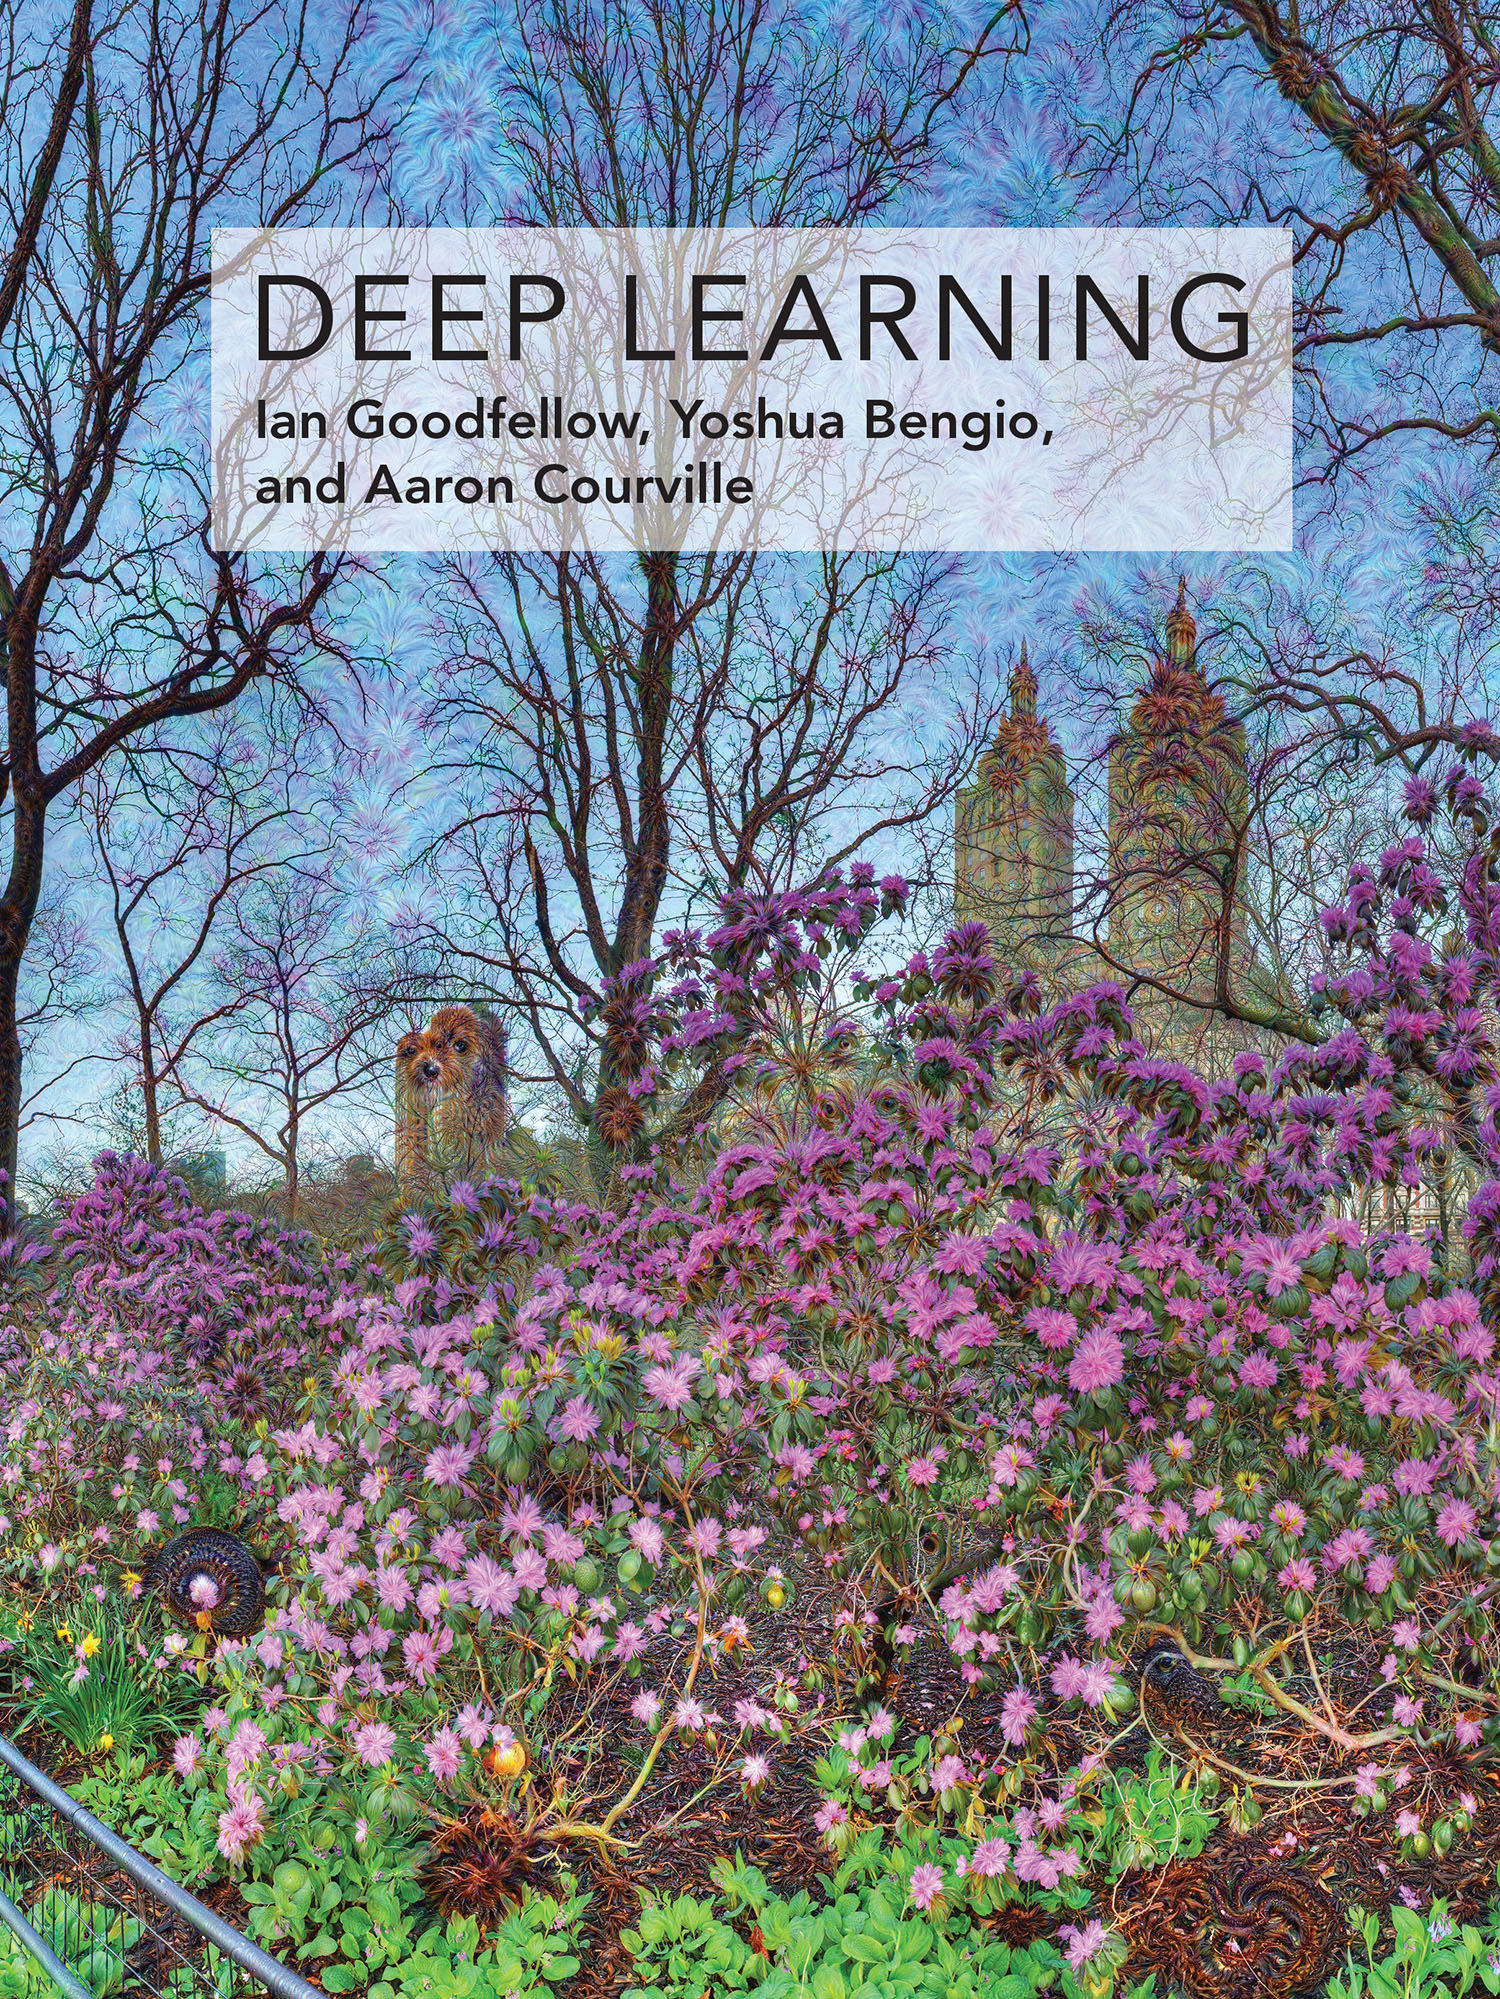
\includegraphics[width=\textwidth]{dl-book.jpg}
\end{minipage}
\begin{minipage}{.49\textwidth}
{\small I. Goodfellow, Y. Bengio, A. Courville}\\
\emph{Deep Learning}\\
MIT Press 2016 \\
\url{www.deeplearningbook.org}
\end{minipage}
\end{frame}
\begin{frame}{Literatura}
\begin{minipage}{.5\textwidth}

\includegraphics[width=\textwidth]{handson.jpg}
\end{minipage}
\begin{minipage}{.49\textwidth}
Aurélien Géron\\
\emph{Hands-On Machine Learning with Scikit-Learn and TensorFlow}\\
O'Reilly Media 2017
\end{minipage}
\end{frame}
\begin{frame}{Plan wykładu}
\begin{enumerate}
\item Regresja liniowa, wielomianowa i logistyczna
\item Warstwowe sieci neuronowe
\item Uczenie ze wzmocnieniem
\end{enumerate}
\end{frame}

\begin{frame}{Program uczący się}
\begin{block}{T. Mitchell \emph{Machine Learning} 1997}
Program komputerowy \emph{uczy się} z doświadczenia $E$ względem pewnej klasy zadań $T$ i miary jakości $P$, jeżeli wartość jego miary jakości $P$ na zadaniach z klasy $T$ poprawia się wraz ze ilością doświadczenia $E$.
\end{block}
\end{frame}

\begin{frame}{Niewyczerpująca lista klas zadań $T$}
\begin{itemize}
\item<+-> klasyfikacja
\item<+-> klasyfikacja z brakującymi wejściami
\item<+-> regresja
\item<+-> transkrypcja
\item<+-> tłumaczenie maszynowe
\item<+-> przewidywanie złożonych struktur
\item<+-> detekcja anomalii
\item<+-> synteza i próbkowanie
\item<+-> uzupełnianie brakujących wejść
\item<+-> usuwanie szumu
\item<+-> estymacja rozkładu prawdopodobieństwa
\end{itemize}
\end{frame}

\begin{frame}{Miary jakości $P$}
\begin{block}{}
Liczbowy sposób określenia jak dobrze/źle program rozwiązuje zadanie $T$.
\end{block}
%TODO zbiór uczący i testowy
%TODO inna miara w procesie uczenia, inna miara w procesie testowania
Bywa prosta do zdefiniowania i obiektywna, np. trafność klasyfikacji \ang{accuracy} w zadaniu \emph{jaka cyfra jest na rysunku}
\[ \frac{\text{odpowiedzi poprawne}}{\text{wszystkie odpowiedzi}} \]
%TODO podzielic na kilka slajdow, dolozyc przyklady nagryzmolonych cyfr
ale również nieobiektywna, np. trafność klasyfikacji w zadaniu \emph{czy ten pasażer jest terrorystą}
\[ \frac{\text{pasażerowie, którzy nie są terrorystami}}{\text{wszyscy pasażerowie}}\approx 100\% \]
albo trudna do zdefiniowania \emph{Grzegorz ma kota}
\begin{enumerate}
\item Grzegorz's got a cat
\item Grzegorz has a cat
\item He has a cat (Google Translate)
\item Gregory has a cat
\end{enumerate}
\end{frame}

\begin{frame}{Doświadczenie $E$}
\begin{itemize}
\item uczenie nadzorowane \ang{supervised}: zbiór przykładów opisanych cechami wraz z etykietami
\item uczenie nienadzorowane \ang{unsupervised}: zbiór przykładów opisanych cechami
\item uczenie ze wzmocnieniem \ang{reinforcement}: środowisko, w którym można wykonywać pewne akcje
\item uczenie częściowo nadzorowane \ang{semi-supervised}: niektóre przykłady mają etykiety
\end{itemize}
\end{frame}

\begin{frame}{Reprezentacja}
Macierz cech $\vec{X}$ mająca $n$ wierszy oraz $p$ kolumn, zwykle liczby rzeczywiste:
\[ \vec{X} = \begin{bmatrix}
X_{1,1} & X_{1,2} & \ldots & X_{1,p} \\
X_{2,1} & X_{2,2} & \ldots & X_{2,p} \\
\vdots & \vdots & \ddots & \vdots \\
X_{n,1} & X_{n,2} & \ldots & X_{n,p} \\
\end{bmatrix} \in \R^{n\times p} \]
\end{frame}

\begin{frame}{Reprezentacja}
Wektor etykiet $\vec{y}$
\[ \vec{y} = \begin{bmatrix}
y_1 \\
y_2 \\
\vdots \\
y_n
\end{bmatrix} \in \R^n \]
\end{frame}

\end{document}
